\section{Qsim::VmQ Class Reference}
\label{classQsim_1_1VmQ}\index{Qsim::VmQ@{Qsim::VmQ}}
{\tt \#include $<$qsim.h$>$}

Collaboration diagram for Qsim::VmQ:\nopagebreak
\begin{figure}[H]
\begin{center}
\leavevmode
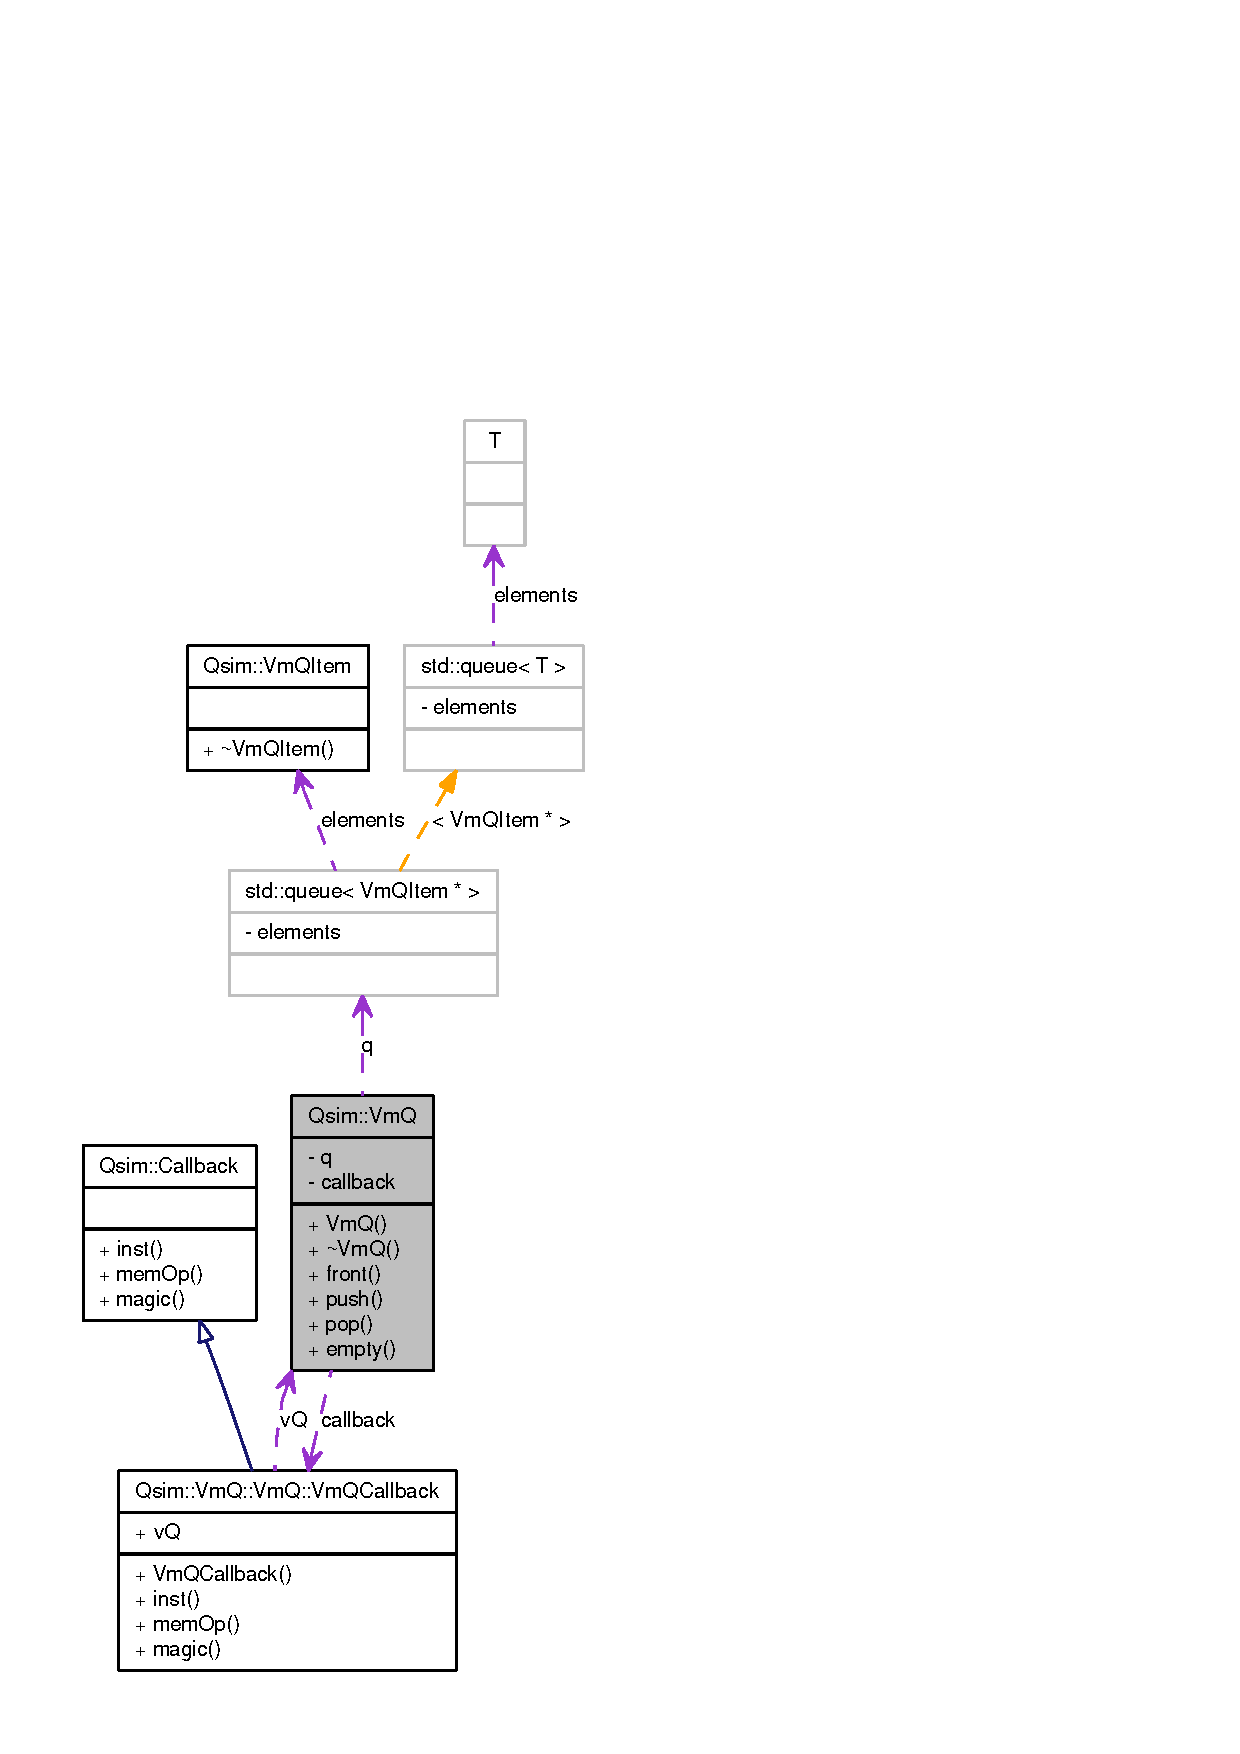
\includegraphics[height=400pt]{classQsim_1_1VmQ__coll__graph}
\end{center}
\end{figure}
\subsection*{Classes}
\begin{CompactItemize}
\item 
class {\bf VmQCallback}
\end{CompactItemize}
\subsection*{Public Member Functions}
\begin{CompactItemize}
\item 
{\bf VmQ} ({\bf Vm} \&v)
\item 
{\bf $\sim$VmQ} ()
\item 
{\bf VmQItem} $\ast$ {\bf front} ()
\item 
void {\bf push} ({\bf VmQItem} $\ast$i)
\item 
void {\bf pop} ()
\item 
bool {\bf empty} ()
\end{CompactItemize}
\subsection*{Private Attributes}
\begin{CompactItemize}
\item 
std::queue$<$ {\bf VmQItem} $\ast$ $>$ {\bf q}
\item 
{\bf VmQCallback} {\bf callback}
\end{CompactItemize}


\subsection{Detailed Description}


Definition at line 119 of file qsim.h.

\subsection{Constructor \& Destructor Documentation}
\index{Qsim::VmQ@{Qsim::VmQ}!VmQ@{VmQ}}
\index{VmQ@{VmQ}!Qsim::VmQ@{Qsim::VmQ}}
\subsubsection[{VmQ}]{\setlength{\rightskip}{0pt plus 5cm}Qsim::VmQ::VmQ ({\bf Vm} \& {\em v})}\label{classQsim_1_1VmQ_fc30b9e3bd54e5d3f25d0c09620a9d3f}


\index{Qsim::VmQ@{Qsim::VmQ}!$\sim$VmQ@{$\sim$VmQ}}
\index{$\sim$VmQ@{$\sim$VmQ}!Qsim::VmQ@{Qsim::VmQ}}
\subsubsection[{$\sim$VmQ}]{\setlength{\rightskip}{0pt plus 5cm}Qsim::VmQ::$\sim$VmQ ()}\label{classQsim_1_1VmQ_b20664e64ffe001fec9ab36920997515}




\subsection{Member Function Documentation}
\index{Qsim::VmQ@{Qsim::VmQ}!empty@{empty}}
\index{empty@{empty}!Qsim::VmQ@{Qsim::VmQ}}
\subsubsection[{empty}]{\setlength{\rightskip}{0pt plus 5cm}bool Qsim::VmQ::empty ()\hspace{0.3cm}{\tt  [inline]}}\label{classQsim_1_1VmQ_5c0c8d1fdb1b1ee77a1e121aab636d46}




Definition at line 127 of file qsim.h.

References q.\index{Qsim::VmQ@{Qsim::VmQ}!front@{front}}
\index{front@{front}!Qsim::VmQ@{Qsim::VmQ}}
\subsubsection[{front}]{\setlength{\rightskip}{0pt plus 5cm}{\bf VmQItem}$\ast$ Qsim::VmQ::front ()\hspace{0.3cm}{\tt  [inline]}}\label{classQsim_1_1VmQ_089c354c8daf95d56e7af7ce58c81a17}




Definition at line 124 of file qsim.h.

References q.\index{Qsim::VmQ@{Qsim::VmQ}!pop@{pop}}
\index{pop@{pop}!Qsim::VmQ@{Qsim::VmQ}}
\subsubsection[{pop}]{\setlength{\rightskip}{0pt plus 5cm}void Qsim::VmQ::pop ()\hspace{0.3cm}{\tt  [inline]}}\label{classQsim_1_1VmQ_97cb4cc44ef2bdebe184ab4273936714}




Definition at line 126 of file qsim.h.

References q.\index{Qsim::VmQ@{Qsim::VmQ}!push@{push}}
\index{push@{push}!Qsim::VmQ@{Qsim::VmQ}}
\subsubsection[{push}]{\setlength{\rightskip}{0pt plus 5cm}void Qsim::VmQ::push ({\bf VmQItem} $\ast$ {\em i})\hspace{0.3cm}{\tt  [inline]}}\label{classQsim_1_1VmQ_024c94a0970fdc29ac670b140541e545}




Definition at line 125 of file qsim.h.

References q.

\subsection{Member Data Documentation}
\index{Qsim::VmQ@{Qsim::VmQ}!callback@{callback}}
\index{callback@{callback}!Qsim::VmQ@{Qsim::VmQ}}
\subsubsection[{callback}]{\setlength{\rightskip}{0pt plus 5cm}{\bf VmQCallback} {\bf Qsim::VmQ::callback}\hspace{0.3cm}{\tt  [private]}}\label{classQsim_1_1VmQ_ff34fcfcd76a885e581a7c46d4b03b1b}




Definition at line 142 of file qsim.h.\index{Qsim::VmQ@{Qsim::VmQ}!q@{q}}
\index{q@{q}!Qsim::VmQ@{Qsim::VmQ}}
\subsubsection[{q}]{\setlength{\rightskip}{0pt plus 5cm}std::queue$<${\bf VmQItem} $\ast$$>$ {\bf Qsim::VmQ::q}\hspace{0.3cm}{\tt  [private]}}\label{classQsim_1_1VmQ_a2f217bc8def898995620e99762243c6}




Definition at line 130 of file qsim.h.

Referenced by empty(), front(), pop(), and push().

The documentation for this class was generated from the following file:\begin{CompactItemize}
\item 
{\bf qsim.h}\end{CompactItemize}
